%!TEX TS-program = pdflatexmk
\documentclass[aspectratio=169]{beamer}

%packages
\usepackage{amsmath,amsthm,amssymb,amsfonts,amsxtra,amstext}
\usepackage{graphicx,float}
\usepackage{media9} %needed for including movies, otherwise comment out
%various figure appearance tweaks:
\usepackage{subcaption}
\captionsetup[subfigure]{labelformat=empty,margin=1ex,justification=raggedright}
\captionsetup[figure]{labelformat=empty}
%table tweaks
\usepackage{multirow}
\usepackage{multicol}
%tikz stuff - can be safely commented out if not using tikz for anything
\usepackage{tikz}
\usetikzlibrary{tikzmark,fit,shapes.geometric,positioning,arrows,arrows.meta}
\tikzstyle{every picture}+=[remember picture]

%add your own graphics path as needed:
%\graphicspath{{../Common/Figures/}{../Common/Logos/}}

%presentation theme and Cornell branding
\usetheme{Frankfurt} %if you don't like the navigation links up top, switch to: \usetheme[]{Madrid}
\DefineNamedColor{named}{CornellRed}{cmyk}{0,1,0.79,0.2} 
\usecolortheme[named=CornellRed]{structure}
\usefonttheme[]{serif}
\setbeamertemplate{navigation symbols}{} %i find these useless. ymmv

%logos
\pgfdeclareimage[height=1.5cm]{culogo}{CULogored}
\pgfdeclareimage[height=0.625cm]{CULogowhite}{CULogowhite}
\pgfdeclareimage[height=1.5cm]{csilogo}{CSI_logo}
\pgfdeclareimage[height=1.5cm]{sioslogo}{SIOSLogo_color_vector}

%let's slap the Cornell logo on everything. branding!
\usepackage[absolute,overlay]{textpos}
\setlength{\TPHorizModule}{1mm}
\setlength{\TPVertModule}{1mm}
\newcommand{\MyLogo}{%
\begin{textblock}{14}(153.0,6.35)
  \pgfuseimage{CULogowhite}
\end{textblock}
}

%\BackgroundPicture creates a full-slide image 
%see below for usage example
\newcommand\BackgroundPicture[3]{%
    \setbeamertemplate{background}{%
    \parbox[c][\paperheight]{\paperwidth}{%
        %\vfill \hfill
 \includegraphics[width=#2\paperwidth,height=#3\paperheight]{#1}
         %\hfill \vfill
      }}}


%useful defs - add your own here
\def\mf{\mathbf}
\def\mb{\mathbb}
\def\mc{\mathcal}
\newcommand{\mfbar}[1]{\mf{\bar{#1}}}
\newcommand{\mfhat}[1]{\mf{\hat{#1}}}
\newcommand{\bdot}[1]{\ensuremath{\dot{\mathbf{#1}}}}
\newcommand{\bhat}[1]{\ensuremath{\hat{\mathbf{#1}}}}
\newcommand{\intd}[1]{\ensuremath{\,\mathrm{d}#1}}
\newcommand{\leftexp}[2]{{\vphantom{#2}}^{#1}\!{#2}}
\newcommand{\leftsub}[2]{{\vphantom{#2}}_{#1}\!{#2}}
\newcommand{\fddt}[1]{\ensuremath{\leftexp{\mathcal{#1}}{\frac{\mathrm{d}}{\mathrm{d}t}}}}
\newcommand{\fdddt}[1]{\ensuremath{\leftexp{\mathcal{#1}}{\frac{\mathrm{d}^2}{\mathrm{d}t^2}}}}
\newcommand{\omegarot}[2]{\ensuremath{\leftexp{\mathcal{#1}}{\boldsymbol{\omega}}^{\mathcal{#2}}}}
\newcommand{\refeq}[1]{Equation  (\ref{#1})} 
\newcommand{\reftable}[1]{Table \ref{#1}}  
\newcommand{\reffig}[1]{Figure \ref{#1}}
\newcommand{\refnum}[1]{Ref.~\citenum{#1}}

%fonts and colors - add own defs here
\setbeamerfont{smalleq}{size=\tiny} 
\definecolor{MyBlue}{cmyk}{0.88, 0.7637,0.0032,0} 
\definecolor{MyRed}{cmyk}{0,0.994,1,0} 
\definecolor{MyGreen}{cmyk}{0.8985,0.3258,1,0.2429} 
\definecolor{MyPurple}{cmyk}{0.7708,0.847,0,0} 
\definecolor{MyGraphite}{cmyk}{0.5973,0.5124,0.5077,0.2013} 

% presentation descriptors
\title[]{Title Goes Here}
\subtitle[]{Subtitle Goes Here}
\author[]{Your Name Here}
%if you don't want logos on the title page (or don't want all of them, modify this:
\institute[]{\pgfuseimage{culogo}\hspace{0.75cm}\pgfuseimage{csilogo}\hspace{0.75cm}\pgfuseimage{sioslogo}}
\date[]{Date Goes Here}
\subject{Talks} %modify as desired

%bib stuff 
\usepackage[backend=bibtex, style=authoryear-comp]{biblatex}
\addbibresource{talkbib} %change to your own bibliography file

%custom cite command - change at will (change tiny to footnotesize to make bigger)
\newcommand{\customcite}[1]{\tiny{\citeauthor{#1}, \citetitle{#1}, \citeyear{#1}}}
\newcommand{\customcitenorm}[1]{{\citeauthor{#1}, \citetitle{#1}, \citeyear{#1}}}

% add a macro that saves its argument
\makeatletter
\newcommand{\footlineextra}[1]{\gdef\insertfootlineextra{#1}}
\newbox\footlineextrabox

% add a beamer template that sets the saved argument in a box.
% The * means that the beamer font and color "footline extra" are automatically added. 
\defbeamertemplate*{footline extra}{default}{
    \begin{beamercolorbox}[ht=2.25ex,dp=1ex,leftskip=1ex,wd=0.95\paperwidth]{footline extra}
    \insertfootlineextra
    %\par\vspace{2.5pt}
    \end{beamercolorbox}
}

\addtobeamertemplate{footline}{%
    % set the box with the extra footline material but make it add no vertical space
    \setbox\footlineextrabox=\vbox{\usebeamertemplate*{footline extra}}
    \vskip -\ht\footlineextrabox
    \vskip -\dp\footlineextrabox
    \box\footlineextrabox%
}

% patch \begin{frame} to reset the footline extra material
\let\beamer@original@frame=\frame
\def\frame{\gdef\insertfootlineextra{}\beamer@original@frame}
\footlineextra{}
\makeatother

%record left margin for making things full-frame
\makeatletter
\newlength\beamerleftmargin
\setlength\beamerleftmargin{\Gm@lmargin}
\makeatother

\begin{document}

\part{Talk}
\frame[plain]{\titlepage
\vfill
\centering
{\tiny You may wish to put auspices statements here, or not}
}

%after the title page, set up slide appearance
\setbeamertemplate{background}{ \setbeamercolor{normal text}{bg=white} }
\addtobeamertemplate{headline}{}{\MyLogo}
\setbeamertemplate{navigation symbols}{\insertframenumber{}/\inserttotalframenumber}

\section{Introduction}
\subsection{Introduction} %note that you need both sections and subsection for the navigation to look good for this 

%here's a normal slide:
\frame{
\frametitle{Slide 1}
 You might have some text here
 
 \footlineextra{You might want to cite a paper here: \customcite{savransky2011parameter}}
}

%here's a slide with a full-width image
\frame{
\frametitle{Slide 2}
\centering
\vspace{-1ex}
\hspace*{-\beamerleftmargin}%
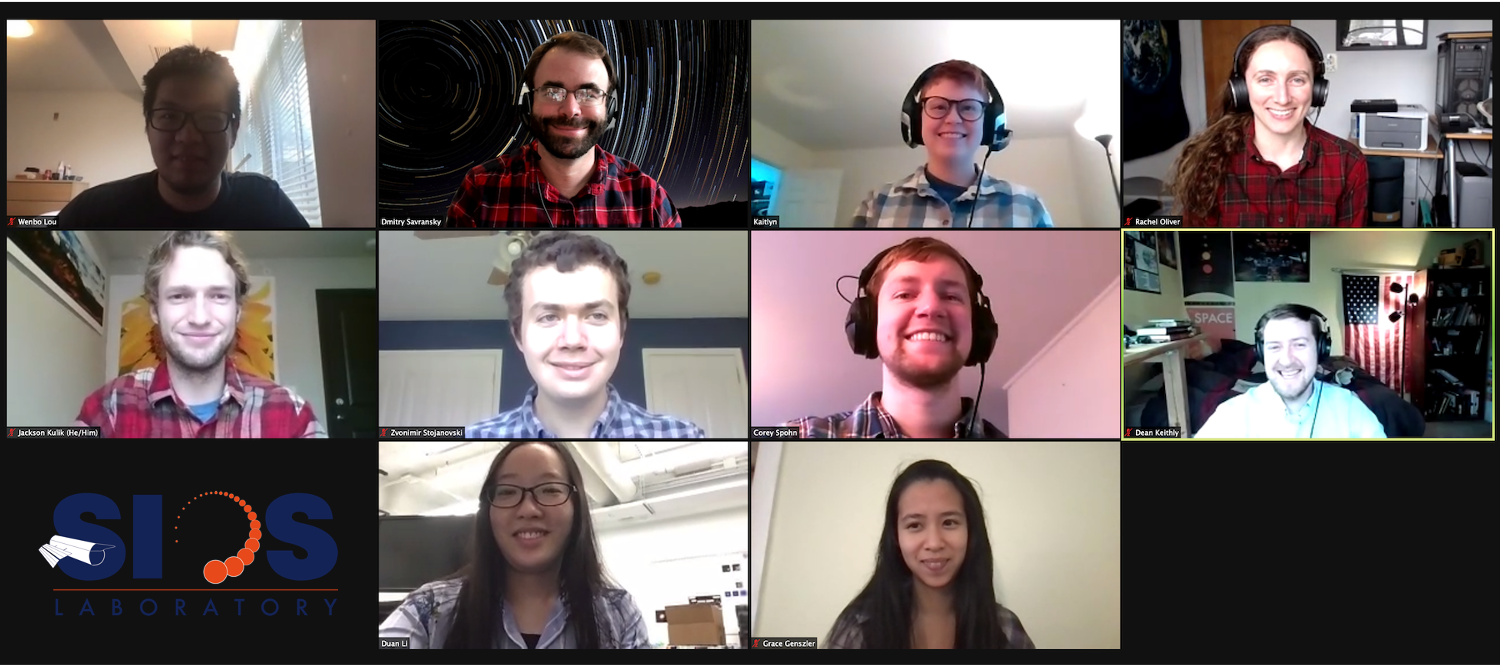
\includegraphics[width=\paperwidth,clip=true,trim= 0in 0in 0in 0in]{labgroup2021}
}

%here's a slide with a full-width image and filled background
{\setbeamercolor{background canvas}{bg=black} 
\frame{
\frametitle{Slide 2}
\centering
\vspace{-1ex}
\hspace*{-\beamerleftmargin}%
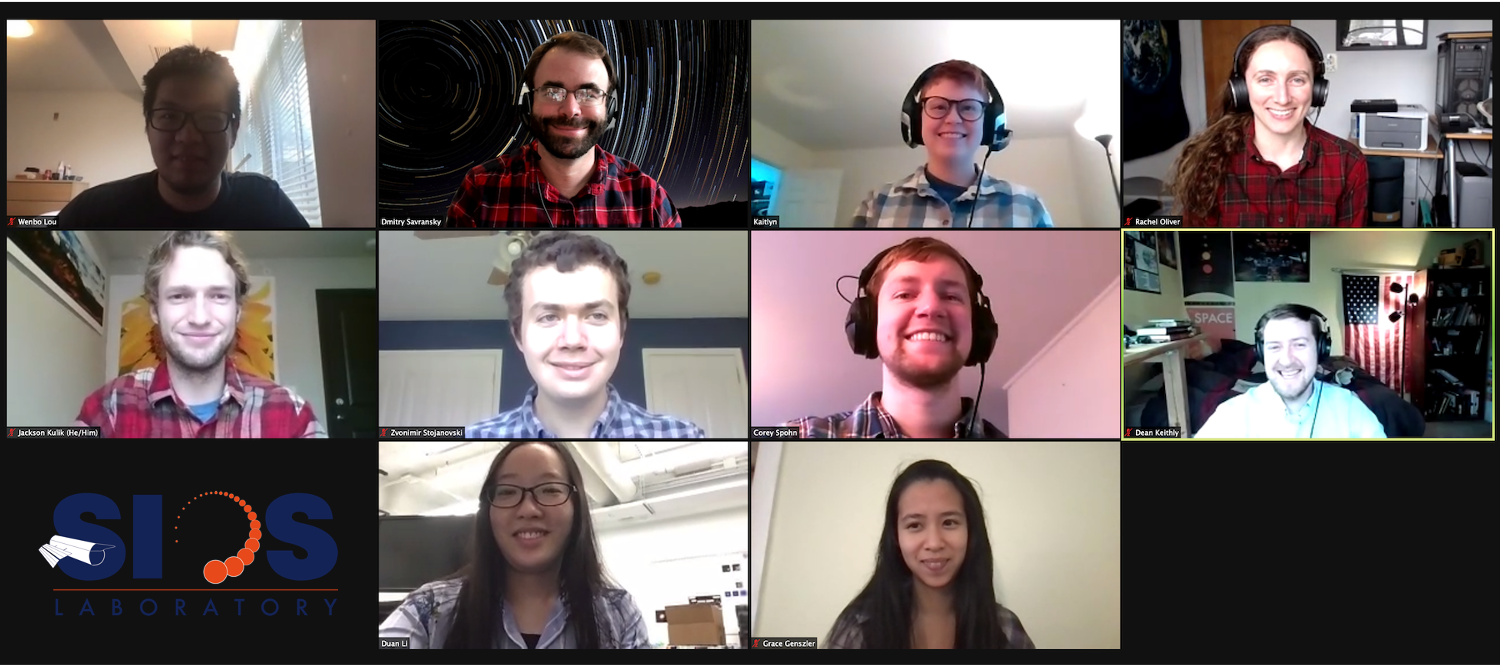
\includegraphics[width=\paperwidth,clip=true,trim= 0in 0in 0in 0in]{labgroup2021}
}}

%here's an example of using the BackgroundPicture and removing any nav symbols
\setbeamertemplate{navigation symbols}{}
\BackgroundPicture{labgroup2021}{1}{0.78} %need to match to image aspect ratio.  these are fractions of 16:9
\frame[plain]{}
 \setbeamertemplate{background}{ \setbeamercolor{normal text}{bg=white} } %put the background back to white
\setbeamertemplate{navigation symbols}{\insertframenumber{}/\inserttotalframenumber} %restore nav symbols

\section{Results}
\subsection{First Result}
%sometimes you'll want to link to a backup slide in case someone has extra questions
\frame[label=mainslide1]{
\frametitle{A Result Slide with Lots of Complexity Behind It}
Here is my amazing result!
\footlineextra{ \hyperlink{backup1}{\beamergotobutton{\tiny{Would You Like to Know More?}}}}
}

%%to include a video (will only play in Adobe Acrobat and a very few other PDF viewers (not macos Preview)
%\frame{
%\frametitle{GPIES}
%
%\includemedia[
%  %width=0.9\linewidth,height=0.675\linewidth, %use this for embedded
%  windowed=1000x500, %use this for floating window
%  activate=pageopen,
%  addresource=filename.mp4, %must be h.264 encoded
%  flashvars={
%     source=filename.mp4 
%    &autoPlay=true
%    &loop=true
%},
%  passcontext
%]{}{VPlayer.swf}
%}
%

%finally, let's compose a complicated slide with a mix of pictures equations and text:
\frame{
\frametitle{Reflected Light}
\begin{picture}(440,210)
\put(-15,-5){
    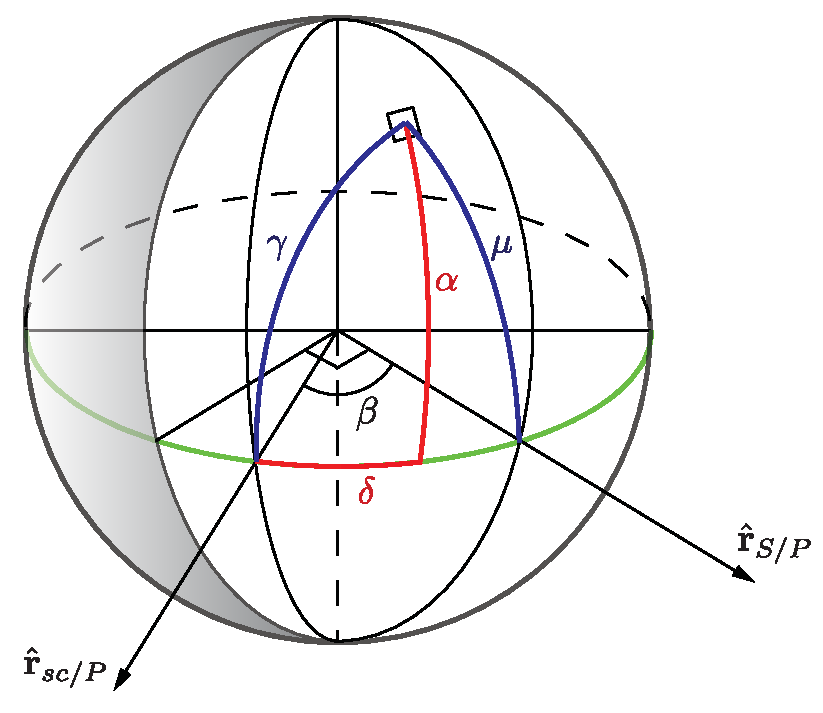
\includegraphics[height=160pt]{reflection_diagram}
}

\put(-10,205){\begin{minipage}[t]{0.6\linewidth}
\small{Energy per second per unit area per unit solid angle received by an observer =}
\vspace{-8pt}
\[ \frac{F R^2}{r^2} \int_{\beta - \pi/2}^{\pi/2} \cos(\beta - \delta) \cos\delta \intd{\delta}  \int_{-\pi/2}^{\pi/2} \rho(C_\mu,C_\gamma,\xi) \cos^3 \alpha \intd{\alpha} \]
\end{minipage}}

\put(110,147){\begin{minipage}[t]{0.4\linewidth}
\small{For isotropic scattering, $\rho$ = constant}
\end{minipage}}
\put(130,150){\begin{minipage}[t]{0.2\linewidth}
\[ \Phi(\beta) = \frac{E(\beta)}{E(0)} =  \]
\end{minipage}}

\put(160,120){\begin{minipage}[t]{0.2\linewidth}\
\[\frac{\sin(\beta)+(\pi-\beta)\cos(\beta)}{\pi} \]
\end{minipage}}

\put(170,90){\begin{minipage}[t]{0.2\linewidth}\
\[\frac{F_p}{F_S} = p\Phi(\beta) \left(\frac{R}{r}\right)^2\]
\end{minipage}}

\end{picture}
}

\section{Conclusions}
\subsection{Conclusions}
\frame{
\frametitle{Conclusions}
In conclusion: Don't forget your conclusions!
}

%let's make an appendix with refs and backup slides
%we don't want to count these in the slide total, so we'll stop counting here
\newcounter{finalframe}
\setcounter{finalframe}{\value{framenumber}}

\appendix

{
\subsection{References}
\frame[allowframebreaks]{
\frametitle{References}
\printbibliography  
}}

%backup slides:
\section{Backup}
\subsection{Backup}

\frame[label=backup1]{
\frametitle{A Backup Slide with Additional Info}
\framesubtitle{ \hyperlink{mainslide1}{\beamerreturnbutton{Return}} }
Lots of nitty-gritty stuff that doesn't belong in the main talk
}


\setcounter{framenumber}{\value{finalframe}} %reset the counter

\end{document}